\documentclass{article}
\usepackage{newspaper}
\date{\today}
\currentvolume{1}
\currentissue{2}
\usepackage{times, graphicx, multicols, caption, lettrine, hyperref, framed}
\hypersetup{colorlinks=true}
\usepackage{capt-of}

%\usepackage{picinpar}
\usepackage{wrapfig}

%%%% quote %%%%
\newcommand{\lowbiglquote}[1][70]{%
  \setbox0=\hbox{\fontsize{#1}{0}\selectfont``}%
  \setlength{\dimen0}{\ht0 - \heightof{A}}%
  \noindent\llap{\smash{\lower\dimen0\box0 }}}

\newcommand{\lowbigrquote}[1][70]{%
  \setbox0=\hbox{\fontsize{#1}{0}\selectfont''}%
  \setlength{\dimen0}{\ht0 - \heightof{A}}%
  \unskip\rlap{\smash{\lower\dimen0\box0 }}}

%%%% fancy quote %%%%
\usepackage{tikz}
\usetikzlibrary{backgrounds}
\makeatletter

\tikzset{%
  fancy quotes/.style={
    text width=\fq@width pt,
    align=justify,
    inner sep=1em,
    anchor=north west,
    minimum width=\textwidth,
  },
  fancy quotes width/.initial={.8\textwidth},
  fancy quotes marks/.style={
    scale=8,
    text=white,
    inner sep=0pt,
  },
  fancy quotes opening/.style={
    fancy quotes marks,
  },
  fancy quotes closing/.style={
    fancy quotes marks,
  },
  fancy quotes background/.style={
    show background rectangle,
    inner frame xsep=0pt,
    background rectangle/.style={
      fill=gray!25,
      rounded corners,
    },
  }
}

\newenvironment{fancyquotes}[1][]{%
\noindent
\tikzpicture[fancy quotes background]
\node[fancy quotes opening,anchor=north west] (fq@ul) at (0,0) {``};
\tikz@scan@one@point\pgfutil@firstofone(fq@ul.east)
\pgfmathsetmacro{\fq@width}{\textwidth - 2*\pgf@x}
\node[fancy quotes,#1] (fq@txt) at (fq@ul.north west) \bgroup}
{\egroup;
\node[overlay,fancy quotes closing,anchor=east] at (fq@txt.south east) {''};
\endtikzpicture}

\makeatother

%%%% wflettrine - dropcap in wrap environment %%%%
\usepackage{helvet}\renewcommand{\familydefault}{\sfdefault}
\usepackage{lettrine}
\usepackage{wrapfig}
\newcounter{cnt}\setcounter{cnt}{0}
\def\t{\stepcounter{cnt}\thecnt. cat sat on the mat. }

\newdimen\tttaa
\newdimen\tttbb

\renewcommand\thepage{\the\numexpr(\value{page}+1)/2\relax}

\makeatletter
\def\merge@ps{\afterassignment\merge@ps@\tttbb}

\def\merge@ps@{\afterassignment\merge@ps@@\tttaa}


\def\merge@ps@@{%
\afterassignment\reset@WF@ps\dimen@\WF@ps\valign
%\showthe\count@
\ifnum\count@>\@ne
\advance\count@\m@ne
\expandafter\merge@ps
\fi
}


\def\reset@WF@ps{\afterassignment\reset@WF@ps@\dimen@ii}

\def\reset@WF@ps@#1\valign{%
\edef\new@wf@ps{\new@wf@ps
  \the\dimexpr\dimen@+\tttbb\relax\space
  \the\dimexpr\dimen@ii-\tttbb\relax\space}%
 \def\WF@ps{#1}}


\newcommand\wflettrine[3][]{%
  \setbox\tw@\hbox{\lettrine[#1]{#2}{#3}\global\let\gtmp\L@parshape}%
  \afterassignment\wf@getoffset\count@\gtmp\hoffset
  \setbox\WF@box\hbox{\kern-\dimen@\box\WF@box\kern\dimen@}%
  \noindent\box\tw@
    \def\new@wf@ps{}%
    \afterassignment\merge@ps\count@\gtmp
    \edef\WF@ps{\new@wf@ps\space\WF@ps}%
    \@@parshape\c@WF@wrappedlines\WF@ps\z@\columnwidth}


\def\wf@getoffset{\afterassignment\wf@get@ffset\dimen@}
\def\wf@get@ffset#1\hoffset{}

\makeatother

%%%%%%%%%  Front matter   %%%%%%%%%%

\begin{document}
\maketitle

\begin{multicols}{2}


\byline{\sc\Large David Defeated Goliath: How did It Happen?}{Ricky Lim}


\begin{wrapfigure}{r}{0.2\textwidth}
    \vspace{-20pt}
    \centering
    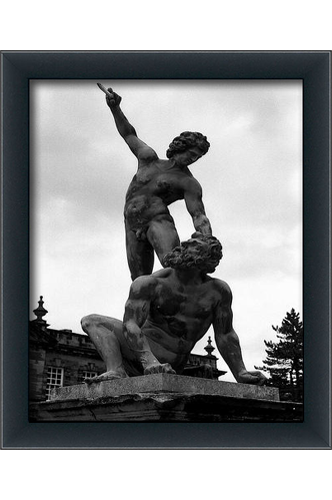
\includegraphics[width=0.15\textwidth]{img/DavidGoliath}
    \vspace{-20pt}
    \caption*{{\small Don't mess up with David}}
  \vspace{-10pt}
\end{wrapfigure}
\wflettrine[lines=3]{H}{ } ere is the very first story of outliers from randomwalk. 
Three \textit{WHYs} I chose a story of \textit{David and Goliath}. 
1). This story invokes lots of different moral \textit{sentiment} given its familiarity.  
2). We might have \textit{misunderstood} this story. 
3). It has awesome \textit{take-home messages.}

\closearticle


\headline{\it\Large Moral sentiments of this story: First Episode.}


First, we gonna get this story \textit{fresh} from its source, which is from the Bible, \textit{1 Sam 17}. 
Because \textit{I'm} a lazy guy, I'm going to use a python code (\textit{./getPassage.py}, available \href{https://github.com/rickylim19/DavidGoliath}{here} on github) to grab this story in three different biblical versions. 
The \textit{NIV} (New International Version), \textit{ESV} (English Standard Version), and \textit{KJV} (King James Version).

Why \textit{we} grabbed these three versions? 
The main reason, \textit{we}'d like to extract different sentiments from this story, given different language perspectives.
I assumed KJV is the \textit{old guy}, NIV represents our \textit{modern translation}, and ESV is somehow in the \textit{middle.}

Having had a collection of these story texts, \textit{I'm} very curious about what's the trend of sentiments along the verses. 
As there are \textit{58 verses} times \textit{3 versions}, so there are \textbf{174} \textit{verses} along the way. 
And \textit{I'm} not going to read and tag my sentiment for each verse (\textit{Hell NO!}). 
So thank God, \textit{we} have our machine that has been \textit{'impressively'} trained to understand the sentiment. 
For this purpose, I used python (./getSentiment.py) to \textit{stream-in} 174 verses into this machine (I used \href{http://web.viralheat.com/sentiment-api/}{Viralheat API} for this analysis) and plotted the sentiment trend in R as a probability of positive and negative sentiments, as shown in figure below.

(*The sentiment analysis report in R is available \href{https://www.dropbox.com/s/q70ip7zgxobbmvt/sentimentPlot.pdf}{here}).

\bigskip
\noindent
\begin{minipage}{\linewidth}
    \centering
    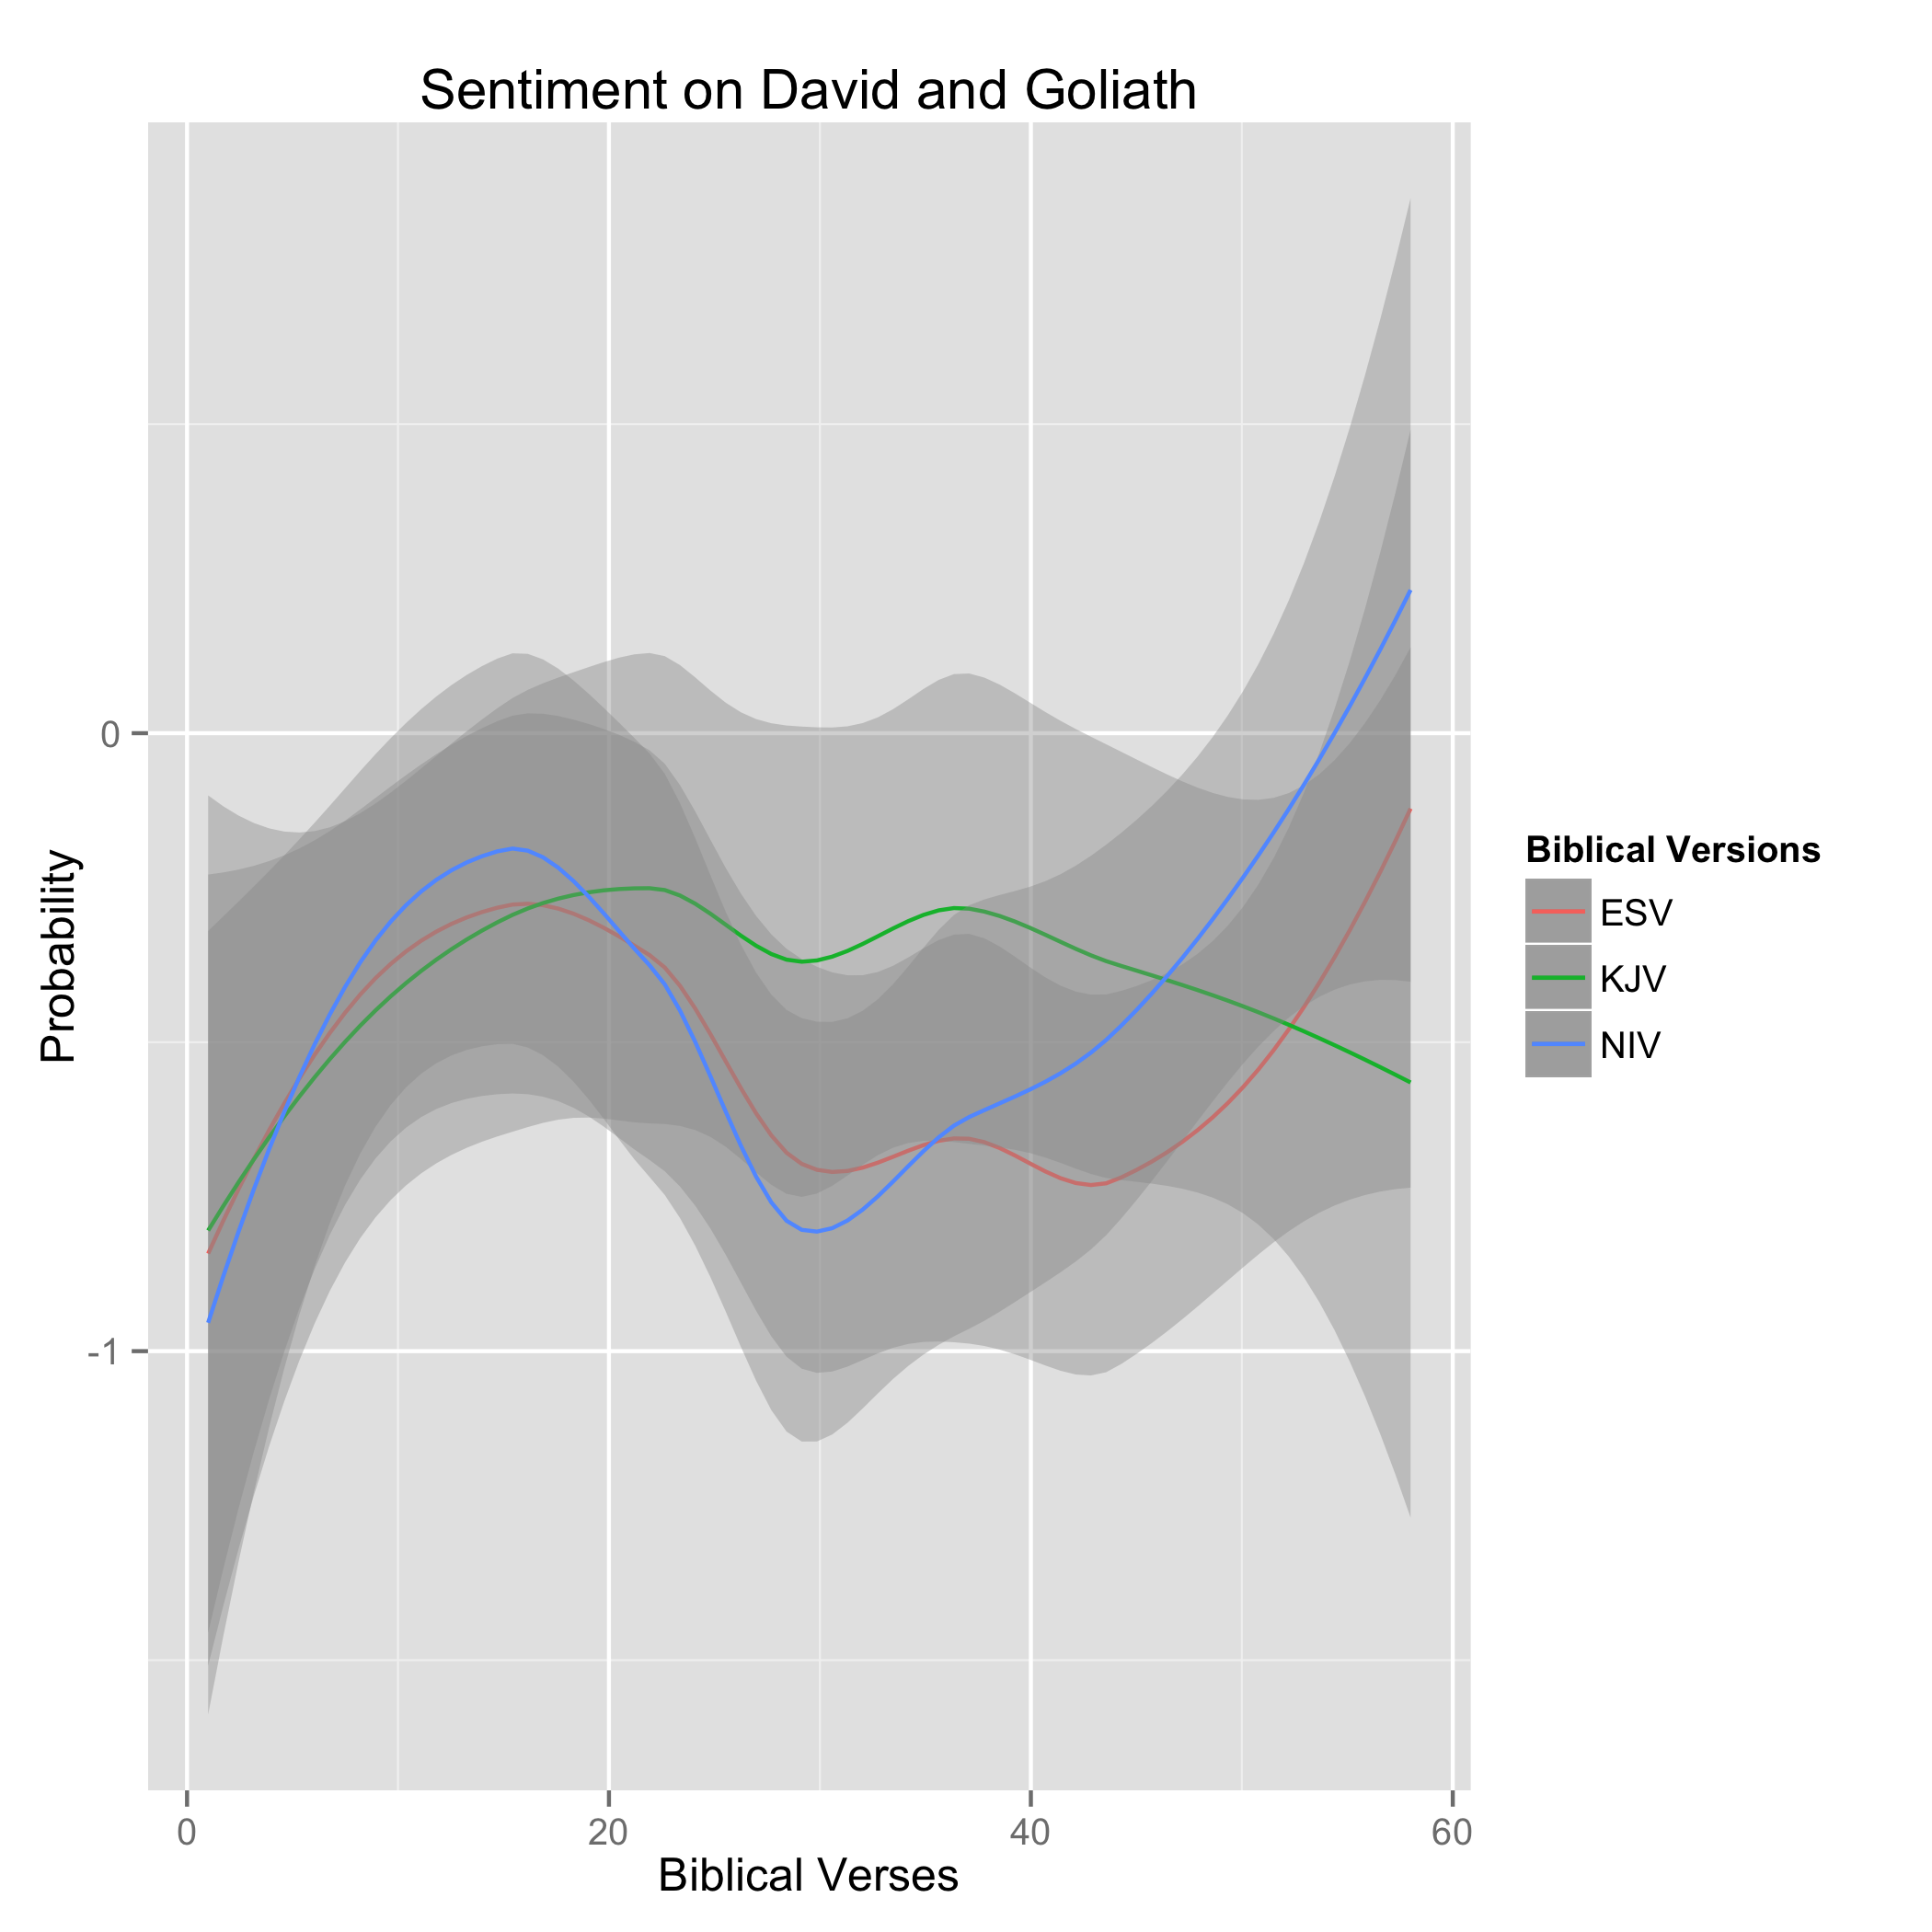
\includegraphics[width=1.\textwidth]{img/sentimentPlot.png}
    \captionof{figure}{{\small Sentiment Trend of David and Goliath. The line was smoothed using loess for a better view.}}

\end{minipage}

\end{multicols}  
\newpage

\begin{multicols}{2}
From figure 1 (above), \textit{we} could see that different biblical versions have their own sentiment trend. 
With our eyes, we could appreciate that the blue (NIV) and the red (ESV) lines show closer fashions one to another (\textit{correlation: 0.69)}. 
Whereas NIV and KJV demonstrate more polar trends with each other (correlation: \textit{0.24}). 
Anyway, the bottom line here is: depending on which version \textit{you} read this story \textit{you} may have different sentiment (that's what this machine wants to say).

Next, I'm going to sum up this story using \textit{Luhn}'s algorithm. 
The core idea behind this guy's algorithm is that the important sentences in a text could be characterized by top occuring words. 
So, I applied this heuristic method to each verse in ESV version (./getSummary.py, available \href{https://github.com/rickylim19/DavidGoliath}{here} on github). 
\textit{Why ESV ?} Because I assumed, this is the standard English so it might be easier to grasp at glance. 
Below is the output.

\textbf{The summary of David and Goliath (ESV):}

\end{multicols}  

\begin{fancyquotes}
  And Saul and the men of Israel were gathered, and encamped in the Valley of Elah, and drew up in line of battle against the Philistines. If he is able to fight with me and kill me, then we will be your servants. But if I prevail against him and kill him, then you shall be our servants and serve us.” And the Philistine said, “I defy the ranks of Israel this day. Give me a man, that we may fight together.” but David went back and forth from Saul to feed his father's sheep at Bethlehem. For forty days the Philistine came forward and took his stand, morning and evening. Also take these ten cheeses to the commander of their thousand. See if your brothers are well, and bring some token from them.” And Israel and the Philistines drew up for battle, army against army. As he talked with them, behold, the champion, the Philistine of Gath, Goliath by name, came up out of the ranks of the Philistines and spoke the same words as before. And David heard him. And the people answered him in the same way, “So shall it be done to the man who kills him.” Your servant has struck down both lions and bears, and this uncircumcised Philistine shall be like one of them, for he has defied the armies of the living God.” and that all this assembly may know that the Lord saves not with sword and spear. For the battle is the Lord 's, and he will give you into our hand.” So David prevailed over the Philistine with a sling and with a stone, and struck the Philistine and killed him. There was no sword in the hand of David. Then David ran and stood over the Philistine and took his sword and drew it out of its sheath and killed him and cut off his head with it. When the Philistines saw that their champion was dead, they fled. And David took the head of the Philistine and brought it to Jerusalem, but he put his armor in his tent.
\end{fancyquotes}

\begin{multicols}{2}
  This summary sounds good enough, \textit{huh}? Thanks to mr.\textit{Luhn} !!. Next I was motivated to parse only very few points from this. So, \textit{I} thought, "how about extracting only the most positive and negative sentiments". From the sentiment analysis, I grabbed only the max and min probability values. (Recall: the higher probability, the more positive the sentiment is and likewise).

  The most \textit{positive} verse in ESV was found at verse 18.

\begin{quotation}
  \lowbiglquote {\small \textit{Also take these ten cheeses to the commander of their thousand. See if your brothers are well, and bring some token from them.}}
\end{quotation}


Interesting \textit{enough}!... although at first glance, I had no idea what it was about. \textit{but}, after contemplating for a little while..\textit{Aha}, it was actually a great verse. It says how David respectfully followed simple and humble commands from his dad (He brought \textit{cheeses} and took care of his brothers!). David was \textit{faithfull} even in small things.. and his reward was yet to come at verse 51 (the one with the most \textit{negative} sentiment!).


\begin{quotation}
  \lowbiglquote {\small \textit{Then David ran and stood over the Philistine and took his sword and drew it out of its sheath and killed him and cut off his head with it. When the Philistines saw that their champion was dead, they fled.}}
\end{quotation}

\textbf{Wooala!}, \textit{he} killed \textit{Goliath} by cutting off his head, coell huh!!, not surprising that this verse was tagged with the most negative one.

So from this simple sentiment analysis on this story, what \textit{we} could learn is: don't expect something \textit{great} to happen, if \textit{you} are not faithful in a very little thing.

\begin{quotation}
  \lowbiglquote {\small \textit{Luke 16:10 ``One who is faithful in a very little is also faithful in much, and one who is dishonest in a very little is also dishonest in much.''}}
\end{quotation}
In the next episode, we gonna learn more how David beats Goliath. Is our metaphor on David as a little guy and Goliath, we like to imagine as a Giant, \textit{right}? Or Are \textit{we} missing something in this story? Stay tune and do \textit{subscribe} this \textit{blog}, and have your say in the comments below!

\textbf{Beer cheers!}
\end{multicols}

\begin{multicols}{2}
\headline{\it \Large Verbs-adverbs and Gladwell exploration in the story of David and Goliath: Second Episode.}

\lettrine[lines=3]{I}{ } t's been quite a while since the first episode, so let's briefly recap the first episode. 
\textit{We} summarized the story based on \textit{Luhn} algorithm and we did a simple sentiment analysis on this story.

From the verses with the most positive and negative sentiment, 
\textit{we} learned that David was \textit{faithful} even in small things that enables him to \textit{defeat} Goliath. 
And we finished the first episode in \textit{question mode}, 
\textit{Is our metaphor on David as a \textbf{little} guy and Goliath as a \textbf{giant}, \textit{right}?}
In this second episode, we will try to deliver an answer, even if it is in no way complete.

\closearticle

David as a little guy often thought as \textit{the underdog} who was less likely to defeat the giant Goliath.
If you grew up going to Sunday School, you're \textit{likelier} to be familiar with such metaphor. 
David-Goliath fight often translates as \textit{good} a metaphor as has ever been made.
So \textit{good}, that \textbf{mr. Gladwell}, in his book \href{http://www.amazon.com/David-Goliath-Underdogs-Misfits-Battling/dp/0316204366}{David and Goliath}, was inspired to challenge it - \textit{Should David have won the battle?}
Here, we will put together the biblical text (ESV version) and mr. Gladwell's provocative thoughts in a version to try to answer: \textit{How \textbf{David} defeated \textbf{Goliath}?}

From the biblical text, we will extract some \textit{keywords} that might help us to understand the story.
Back in elementary school, we were taught about some word categories including \textit{nouns}, \textit{adjectives}, \textit{verbs}, and \textit{adverbs}.
And we've learnt that these categories are useful to process the language. 

Armed with our elementary degree, we will put into practice a simple analysis of the distribution of word categories in the biblical text.
Our simple analysis consists of \textit{tagging} the words, such as \textit{('different', 'adjective')} and \textit{counting} the frequency of the tags.
For simplicity, we will use \href{http://nltk.org/}{NLTK} in python, implemented \href{https://github.com/rickylim19/DavidGoliath}{here, (./getWordFreq4Tag.py)}. 

To answer a \textit{How} question in \textbf{David-Goliath} fight, we will first focus on the \textit{verbs}.
The result of our simple analysis is shown with \href{http://www.wordle.net/}{wordle} (figure 2).
The top three most occurring verbs consist of ``\textbf{went}'', ``\textbf{took}'', and ``\textbf{come}''. 
From these top \textbf{three} verbs, we'll try to learn \textit{how did David defeat Goliath?}

\begin{itemize}
    \item \textbf{Went}. {``\small \textit{David went back and forth from Saul to feed his father's sheep at Bethlehem.''}}\\
        This verse introduced David as a \textit{shepherd}. 
        Being a shepherd means that his job was not only to \textit{lead} his flock to pasture but also to \textit{protect} them against a lion or a bear.
        We learned that David had been equipped with valuable battle experience in wild setting. 

      \item \textbf{Took}. {``\small \textit{Then he took his staff in his hand and chose five smooth stones from the brook and put them in his shepherd's pouch. His sling was in his hand, and he approached the Philistine.''}}\\
          Here is the most interesting part with provocative ideas from mr. Gladwell. 
          In \textit{David-Goliath} fight, 
          Goliath was a warrior. His rank was infantry in ancient armies.
          He was equipped with swords and shields and he expected a duel with another infantryman with swords.  
          This implies a close-combat rule.
          Saul also played with the tacit rule, so he tried to give David his sword and armor. 
          But David \textit{broke} the rule (he gave a sh*t to the rule!).  
          Instead, \textit{he} used the same weapons he used to kill the lion and the bear.
          ``David approached the battle with a \textit{sling} in his hand not with a sword.''
          Without heavy armor and sword, David gains \textit{speed} and a sling serves as surprising \textit{strength} at long-range.


      \item \textbf{Came}. {``\small \textit{Am I a dog, that you come to me with sticks?''}}\\
           In this verse, the bible tried to reveal Goliath's vulnerability. 
           As we read previously David took his \textit{staff}, indicating a singular form. 
           Whereas, the bible recorded what Goliath saw it as \textit{stick\textbf{s}}, not a \textit{stick}.
           This suggests that Goliath might have had \href{http://en.wikipedia.org/wiki/Acromegaly}{acromegaly}, a growth disorder that might have created loss of \textit{vision}.
           Another verse supporting that Goliath was a disabled giant is found in verse 41, 
           \textit{``And the Philistine moved forward and came near to David, \textbf{with his shield-bearer in front of him}''.}
           Goliath came to David with a guy (his shield-bearer) to help him. 
           \textit{Was he not strong enough as a giant to bear a shield?} 
           Or he felt the need to be accompanied to come to David, suggesting something wrong with his vision. 
           Or he just needed a guy to protect him.
           This giant, so called a champion, was not as perfect as they seem after all.
           With such weakness, David was in \textit{situation excellent} to attack and eventually led to victory.\\
\end{itemize}



\begingroup
    \centering
    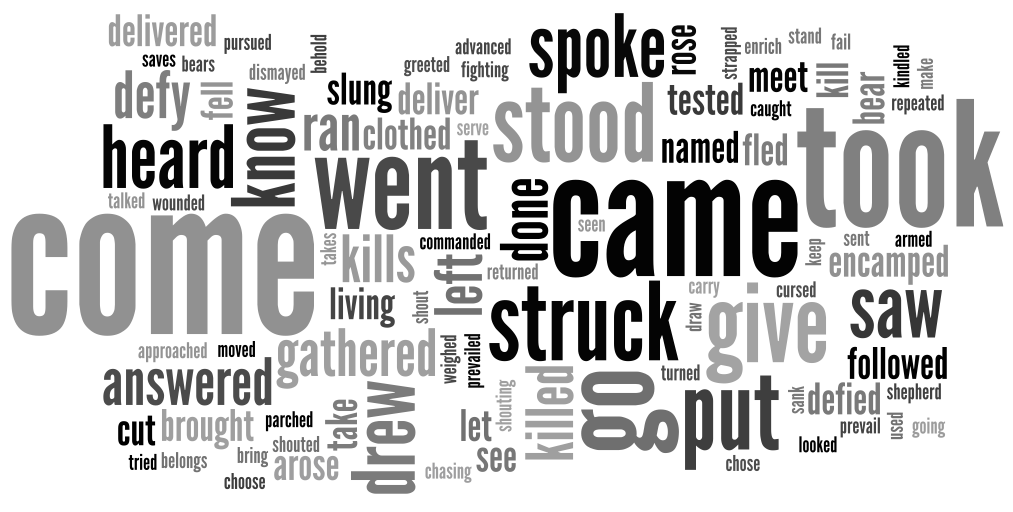
\includegraphics[width=.45\textwidth]{img/verb_ESV.png}
    \captionof{figure}{{\small Verb cloud from 1 Sam 17 (ESV). The size of each verb is scaled according to its frequency of occurance. (The word ``Said'' serves as a control for a storical text and being excluded in this cloud.)}}
    \vspace{20pt}
\endgroup

What went wrong with such metaphor is we often see it as Saul and the Israelites saw the battle.
We were fooled by the physical appearance. 
David as a little lad makes him less probable to win against the giant Goliath.
But we often fail to see the power in other forms. 
\textit{Should David have won the battle?}
David was not just a lad herding flocks of sheep, but he's also a slinger.
He knew how to win battles in the wild.
Moreover, he seems to face a giant with vision problems which makes David's victory more probable. 
\textit{So whenever you got a chance to tell this battle to the Sunday School kids, please don't get them wrong.} 

The take-home messages that we could extract from this ancient story when we face our giant:
\begin{itemize}
    \item \textbf{Go} out into the battle not to run away. Here where our faith is put into practice.
    \item \textbf{Take} what we're good at. Stop following the rule, follow your instincts and exploit your skills, instead. 
    \item \textbf{Come} to understand your giant's vulnerability. \textit{Nobody is perfect even a giant.}
\end{itemize}

\begingroup
    \centering
    
\includegraphics[width=.45\textwidth]{img/adverb_ESV.png}
    \captionof{figure}{{\small Adverb cloud from 1 Sam 17 (ESV). The frequency of occurance is translated into the size of each adverb. (``Then'' was not shown in this cloud as it serves as a control in the story-telling context.)}}
    \vspace{20pt}
\endgroup

In addition to verb, I also did the analysis for adverbs, as visualized in figure 3.
Throughout this text, ``\textbf{Now}'' was found very frequent.
And ``\textbf{Now}'' may serve to specify the manner how we could defeat our giant. 
Our giant might look very intimidating, but whatever our giant is, decide to defeat it ``\textbf{Now}''.
And I'd like to finish off this blog post with a blockquote.




\end{multicols}

\begin{fancyquotes}
    Stop sucking \textbf{now} and be legendary \textit{instead}! Why \textbf{now}? because \textbf{later} is such crap and when you decide to do it \textbf{now}, it is your lucky moment. -{\small inspired by \href{http://www.codinghorror.com/blog/2012/05/how-to-stop-sucking-and-be-awesome-instead.html}{Coding Horror} and japanese proverb.}
\end{fancyquotes}

\end{document}

